%%% ====================== %%%
%%%      INTRODUCTION      %%%
%%% ====================== %%%

% FIGURE 0-01 - LENGTH SCALES IN ATMOSPHERIC SCIENCES

\begin{figure}
\centering
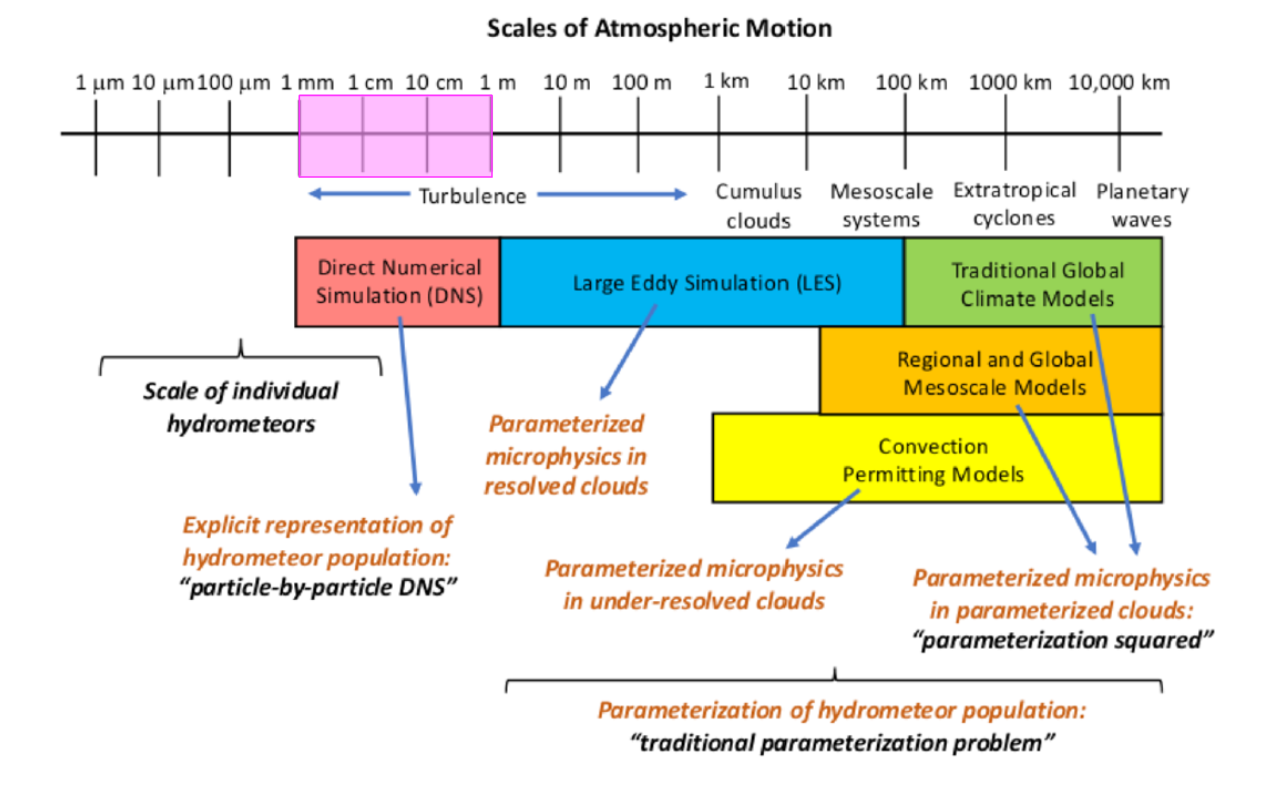
\includegraphics[width=13cm]{figures/0-01_atmo-scales.png}
\caption{
Hierarchy of atmospheric models and the scales of atmospheric motion reproduced from \textcite{Morrison2020} with author's permission.
Coloured rectangles represent types of simulations commonly used when working with respective length scales, and comments emphasise transition from directly resolving most elements of the model (left) to including more and more parameterisations with the increase of scale (right).
Magenta rectangle positioned on the axis was added to emphasise range of scales that corresponds to simulations discussed in this thesis.}
\label{fig:atmo-scales}
\end{figure}



%%% =================== %%%
%%%      CHAPTER 1      %%%
%%% =================== %%%

% FIGURE 1-01 - DETERMINISTIC FORCING ENERGY SPECTRUM

\begin{figure}
\centering
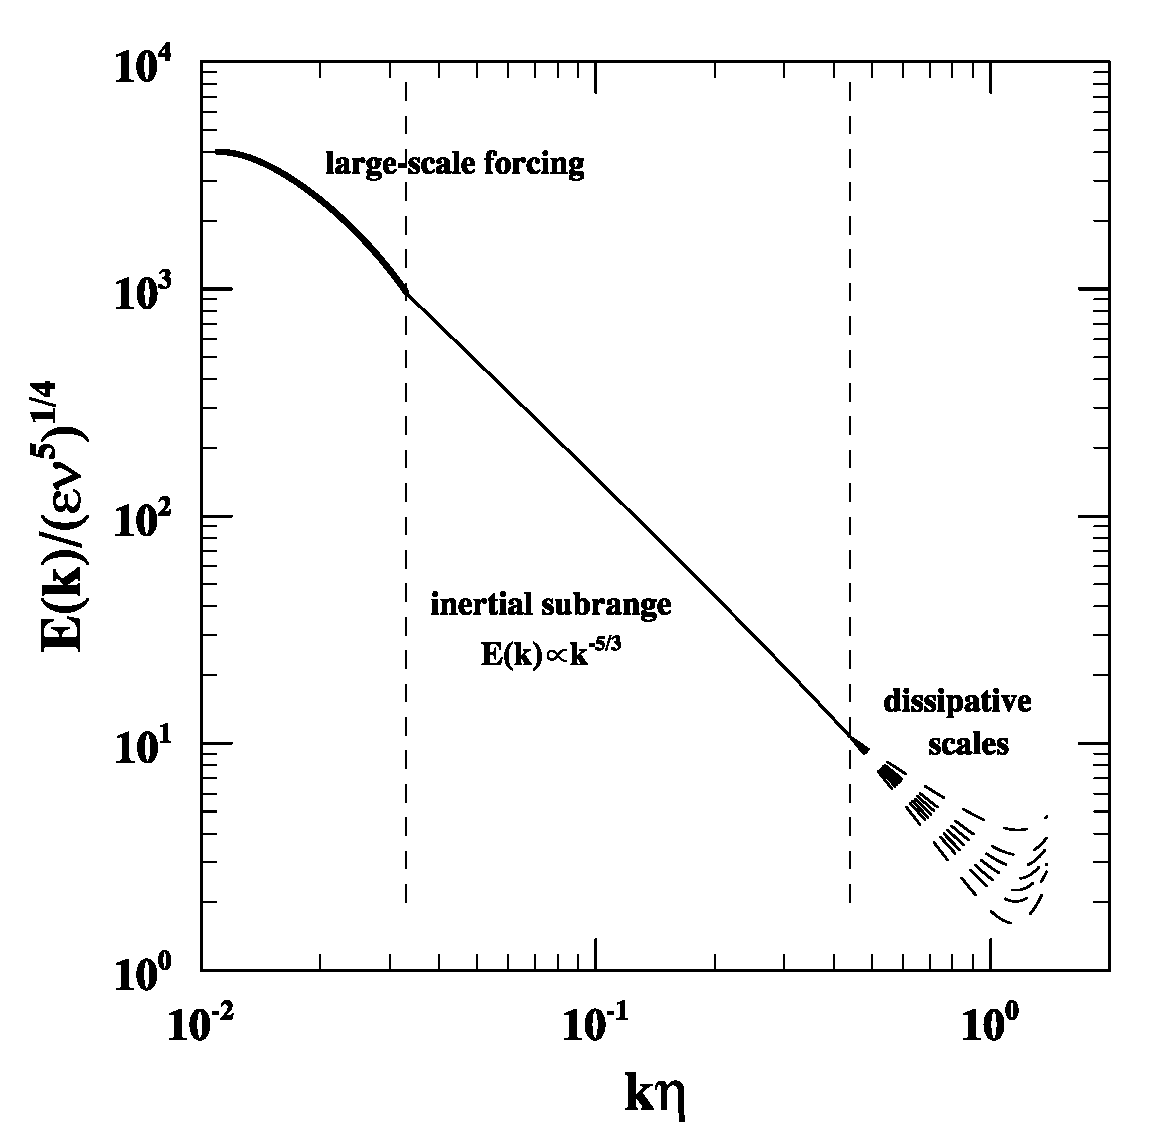
\includegraphics[width=10cm]{figures/1-01_forcing.pdf}
\caption{
The basic idea of deterministic forcing scheme: energy is supplied on large scales by fixing it for small wavenumbers (bold line), then it is transferred following Kolmogorov energy cascade ($E(k) \propto k^{-5/3}$) in inertial subrange, to finally reach smallest dissipative eddies represented by largest resolved wavenumbers (when $k_{\max} \eta \sim 1 = 10^0$, diverging dashed lines) that have largest influence on measured particle statistics at contact distances.
Both axes are using standard normalisations (see Section \ref{ssc:ch2.flow.spec}) and logarithmic scale, that makes $k^{-5/3}$ curves appear as straight lines.}
\label{fig:forcing}
\end{figure}

% FIGURE 1-02 - GRID SIZES IN DNS VS LES

\begin{figure}
\centering
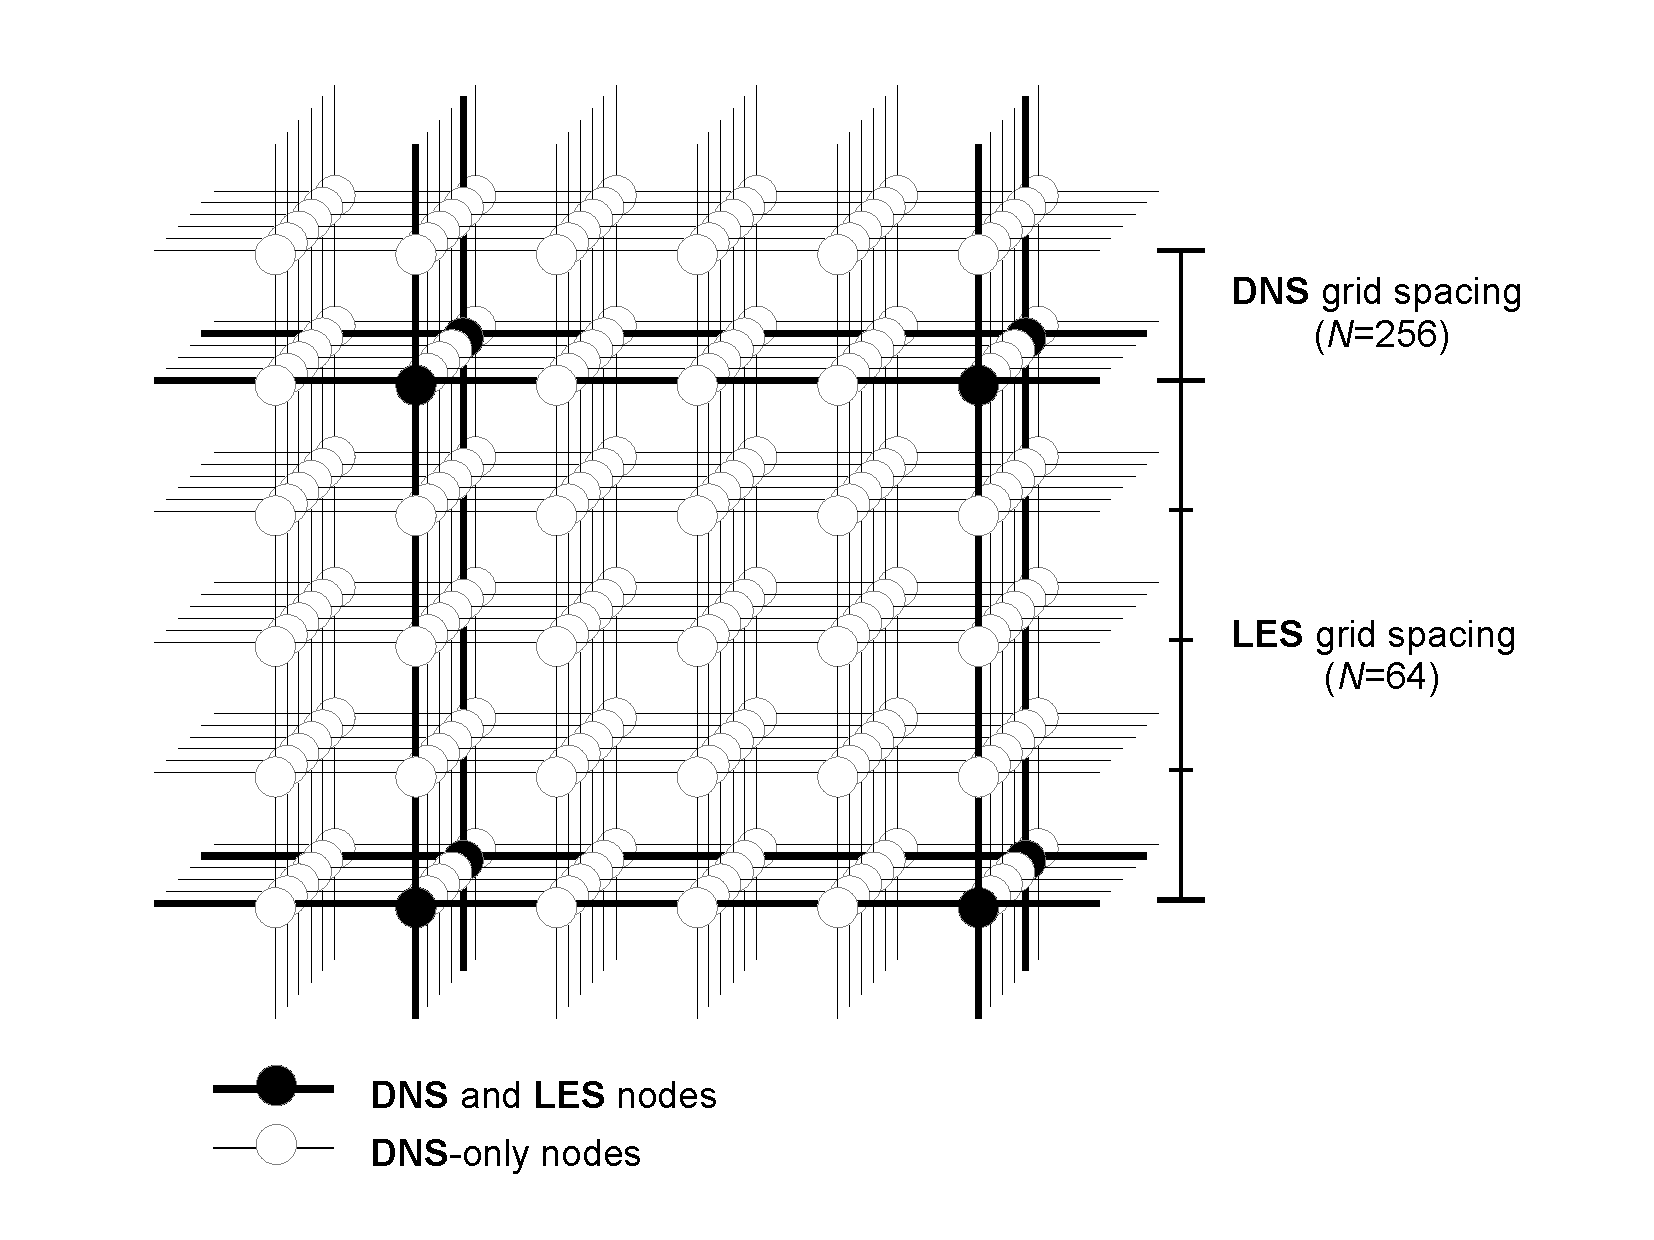
\includegraphics[width=17cm]{figures/1-02_dns-les-grids.pdf}
\caption{
Conceptual juxtaposition of computational grids for DNS and LES.
In LES, the subgrid-scale modelling parameterises small-scale turbulence that is directly resolved by $4 \times 4 \times 4$ block of cells in DNS.
}
\label{fig:dns-les-grids}
\end{figure}

% FIGURE 1-03 - PROJECTION ONTO NEIGHBOURING NODES

\begin{figure}
\centering
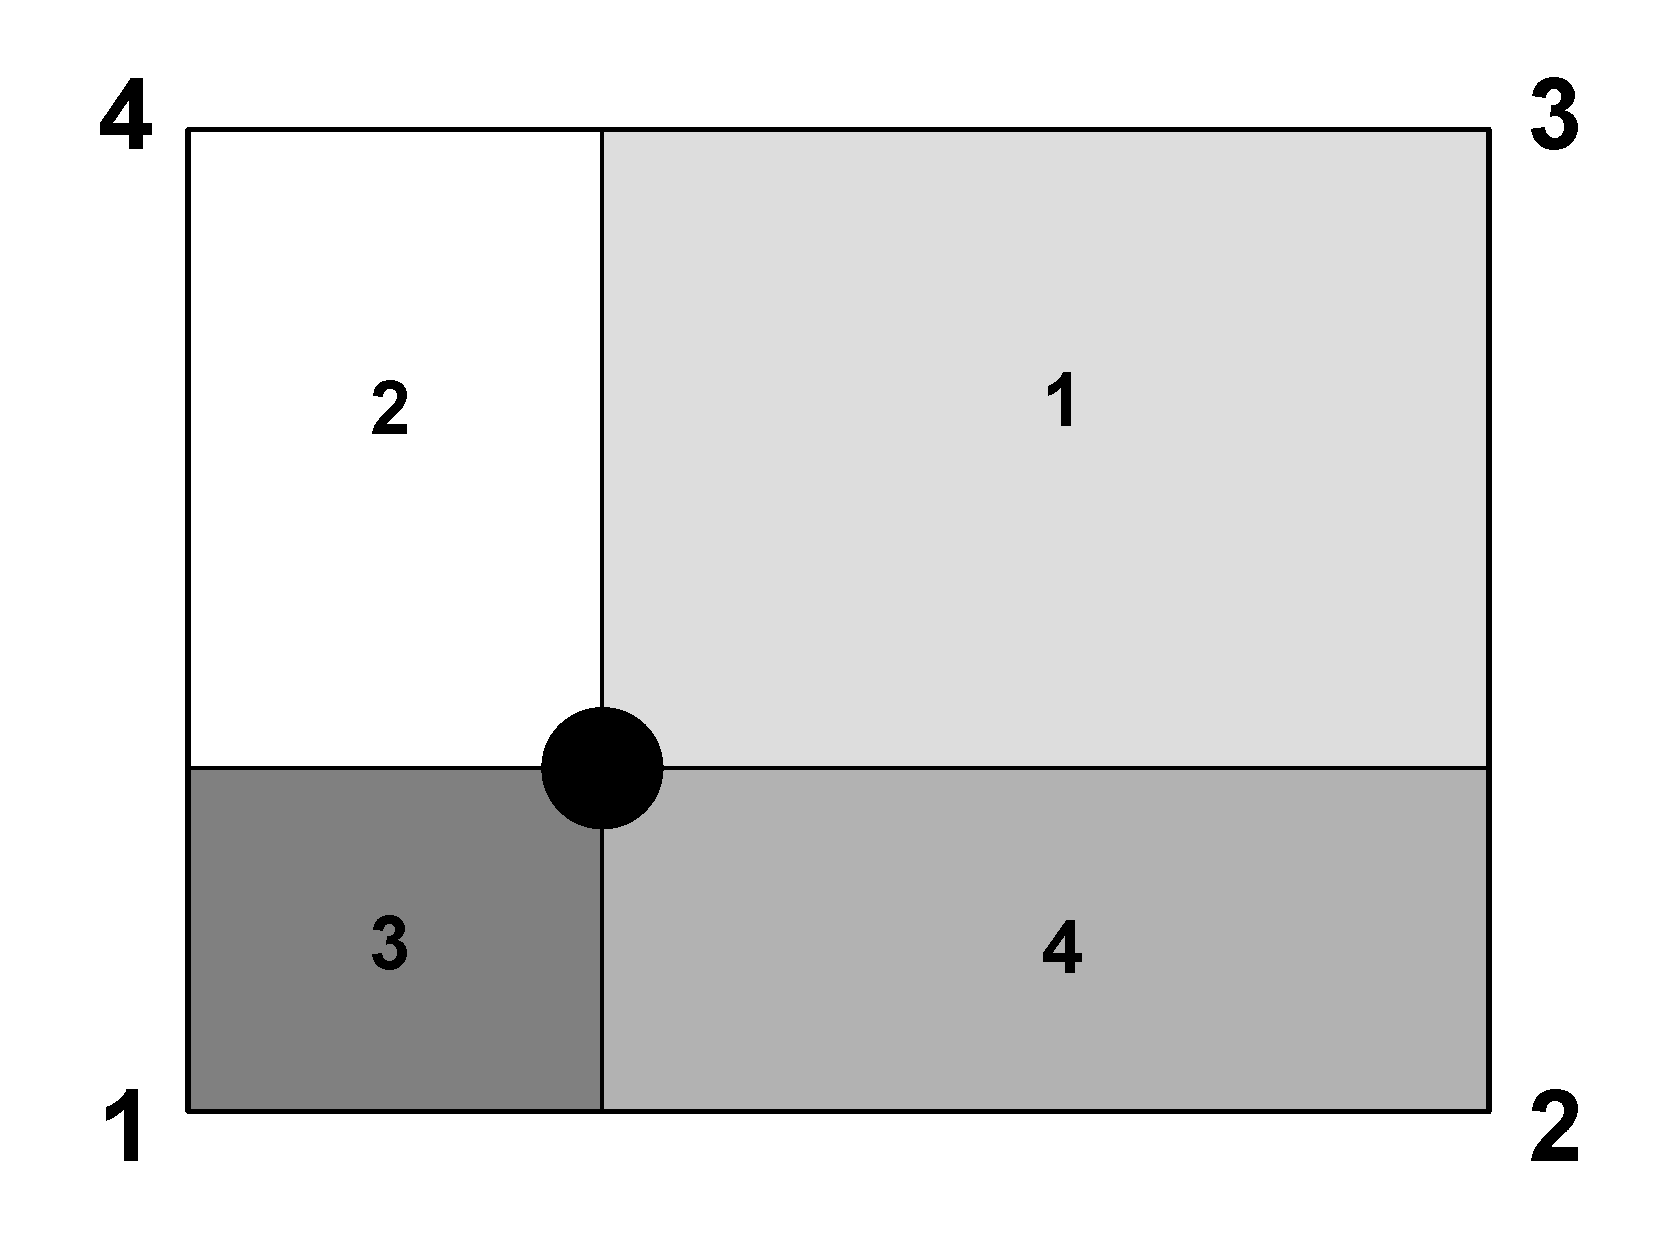
\includegraphics[width=8cm]{figures/1-03_pnn.pdf}
\caption{
Projection onto neighbouring nodes (PNN; simplified illustration for 2D case).
The contribution of the particle momentum to the fluid momentum at a grid node depends on the separation distance.
For example, the particle force may be projected onto neighbouring nodes using weights that are proportional to cell areas (or volumes in 3D case).
Here, the fluid flow at grid node $1$ is affected by a fraction of the particle Stokes drag proportional to the area with marker $1$, and so on.
Based on \textcite[Fig. 1 therein]{Garg2007}.}
\label{fig:pnn}
\end{figure}

% FIGURE 1-04 - 2D DOMAIN DECOMPOSITION

\begin{figure}
\centering
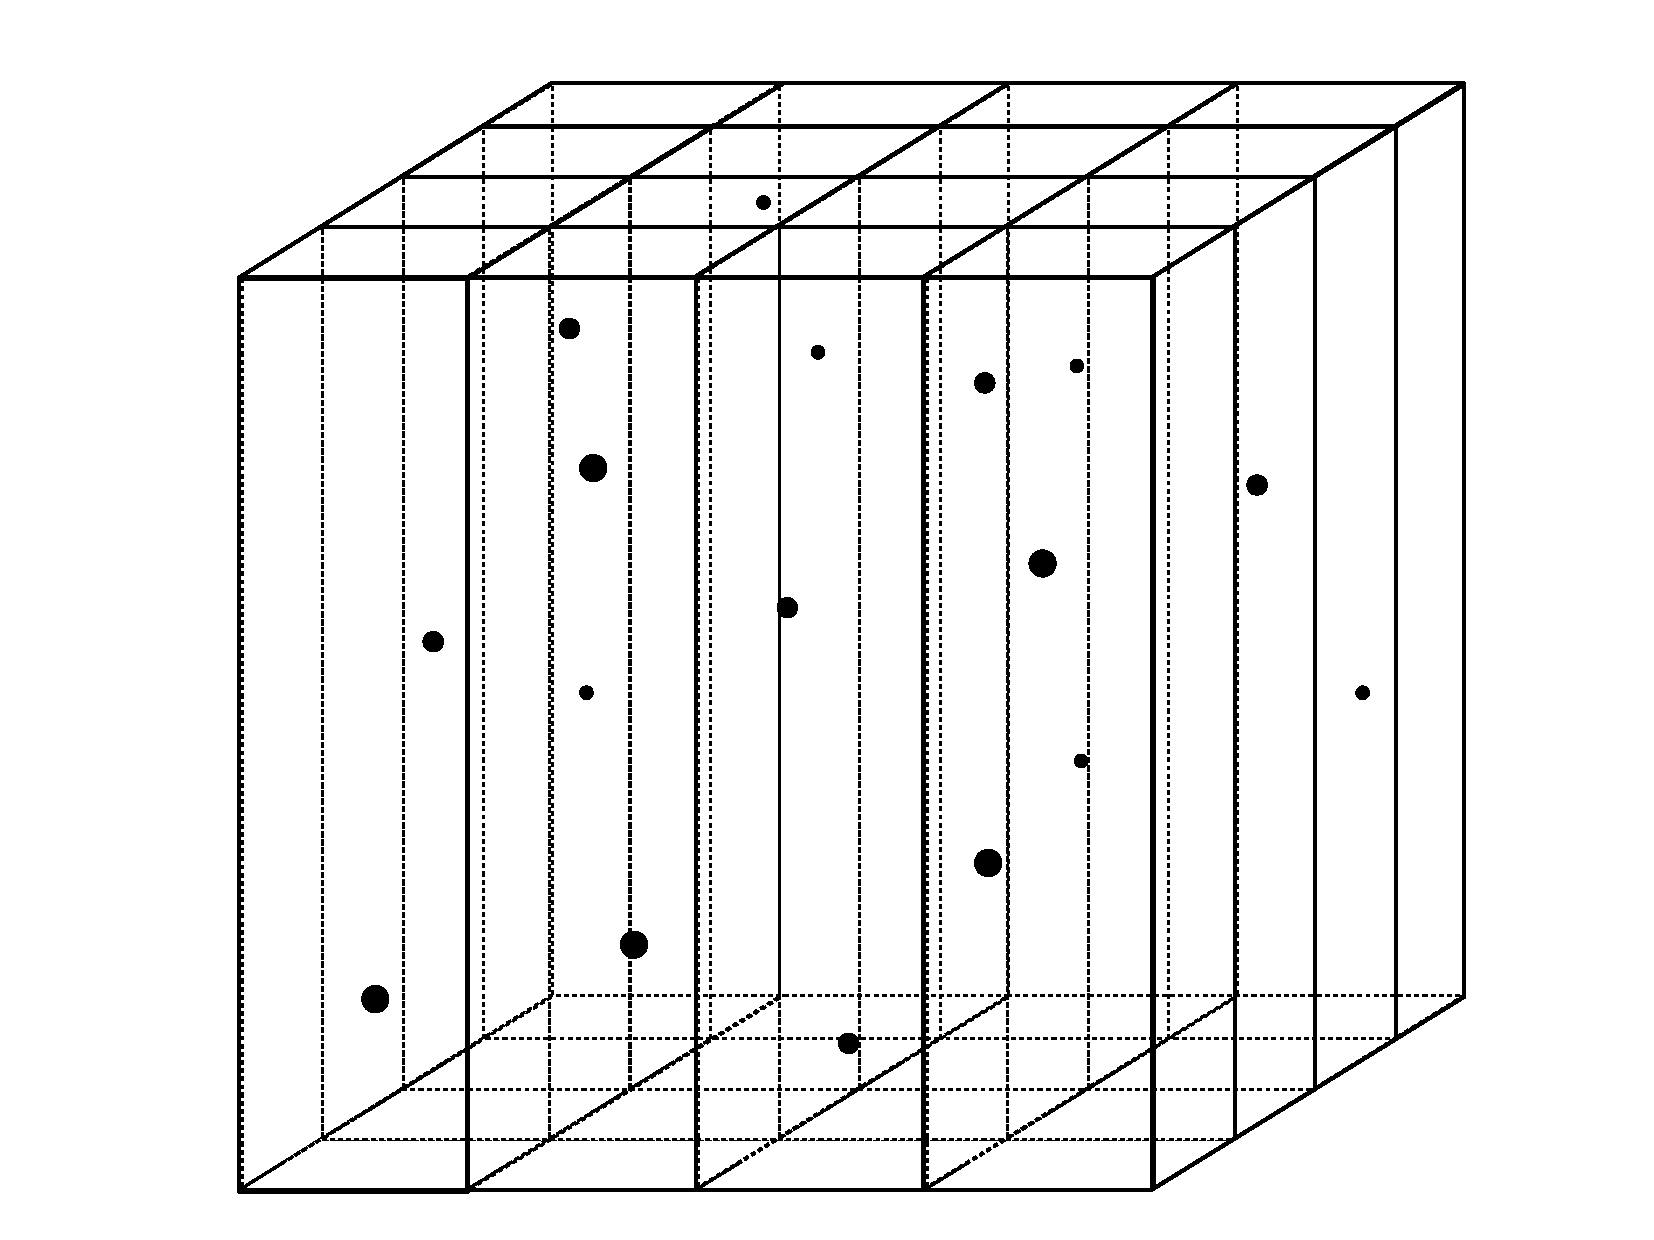
\includegraphics[width=10cm]{figures/1-04_2dd.pdf}
\caption{
Schematic representation of 2D domain decomposition.
This image corresponds to the actual decomposition of $64^{3}$ grid used for LES.
Entire domain is divided into $4 \times 4 = 16$ subdomains, each~with~$16 \times 16 \times 64$ nodes.
}
\label{fig:2dd}
\end{figure}



%%% =================== %%%
%%%      CHAPTER 2      %%%
%%% =================== %%%

% FIGURE 2-01 - TURBULENT FLOW ENERGY SPECTRA

\begin{figure}
\centering
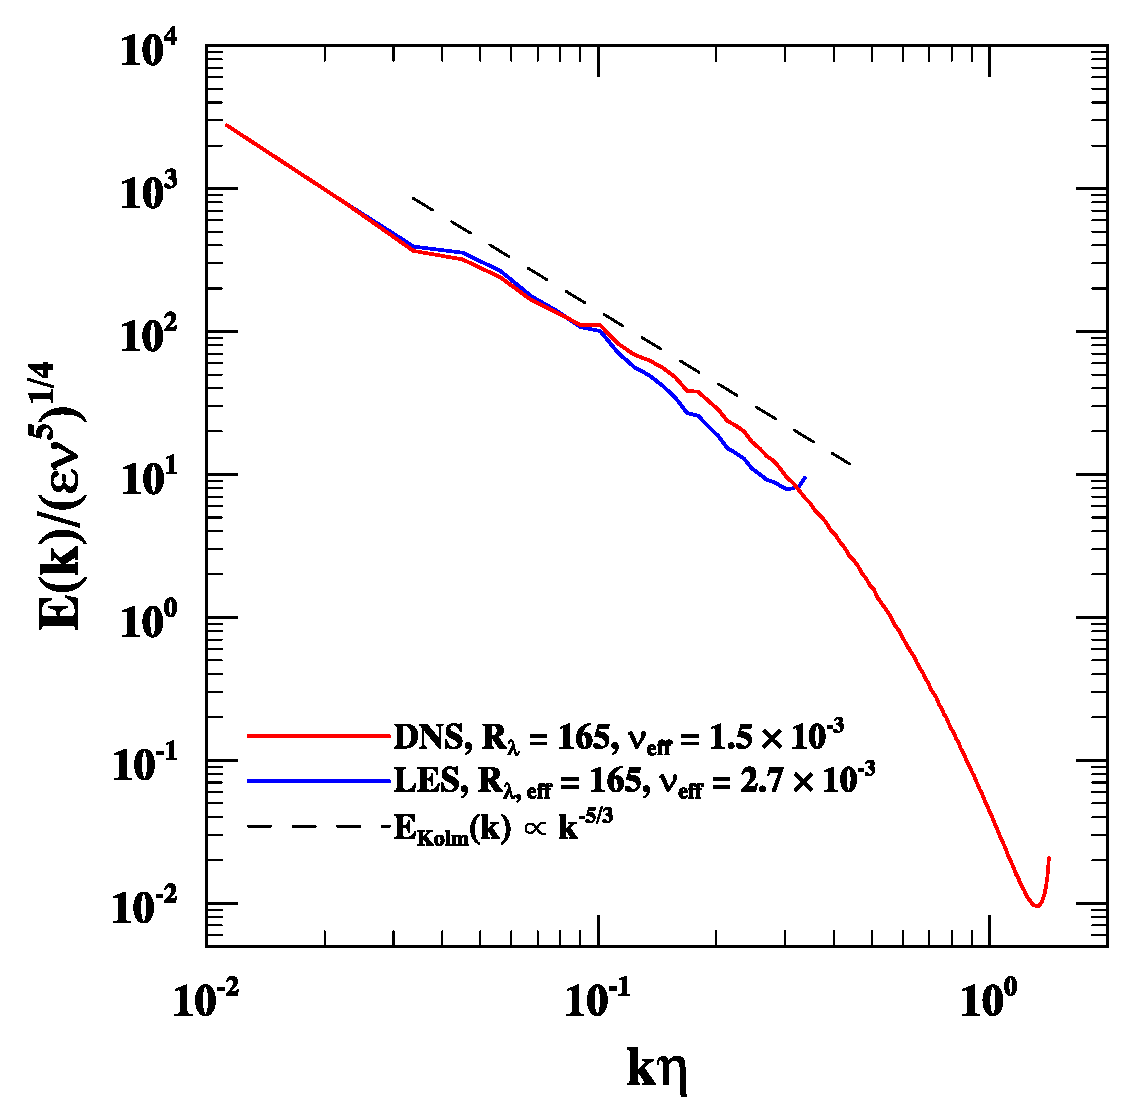
\includegraphics[width=8cm]{figures/2-01_spec.pdf}
\caption{
The normalised energy spectra of background turbulent flows for both DNS and LES.
Dashed line provides comparison with $k^{-5/3}$ curve of theoretical Kolmogorov spectrum (see Equation~\ref{eqn:kolm}) for inertial subrange.
}
\label{fig:spec}
\end{figure}
    
% FIGURE 2-02 - TURBULENT FLOW DISSIPATION SPECTRA

\begin{figure}
\centering
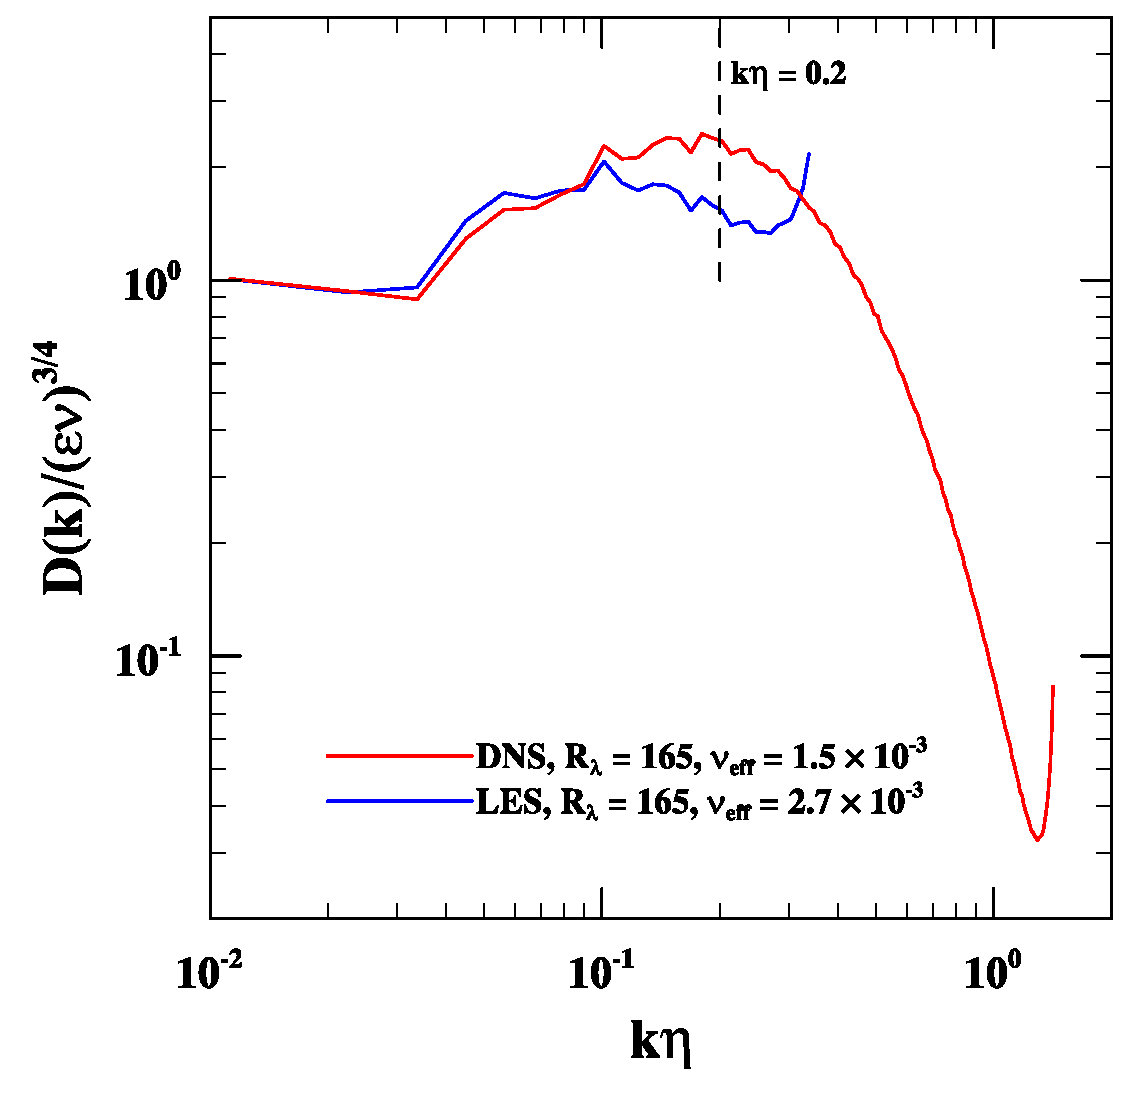
\includegraphics[width=8cm]{figures/2-02_diss.pdf}
\caption{
The normalised energy dissipation spectra of background turbulent flows for both DNS and LES.
Point where $D(k)$ is expected to be maximal (for $k \eta = 0.2$) is marked by dashed line. 
}
\label{fig:diss}
\end{figure}

% FIGURE 2-03 - ENERGY SPECTRA OF TURBULENT FLOWS MODULATED BY PARTICLES

\begin{figure}
\centering
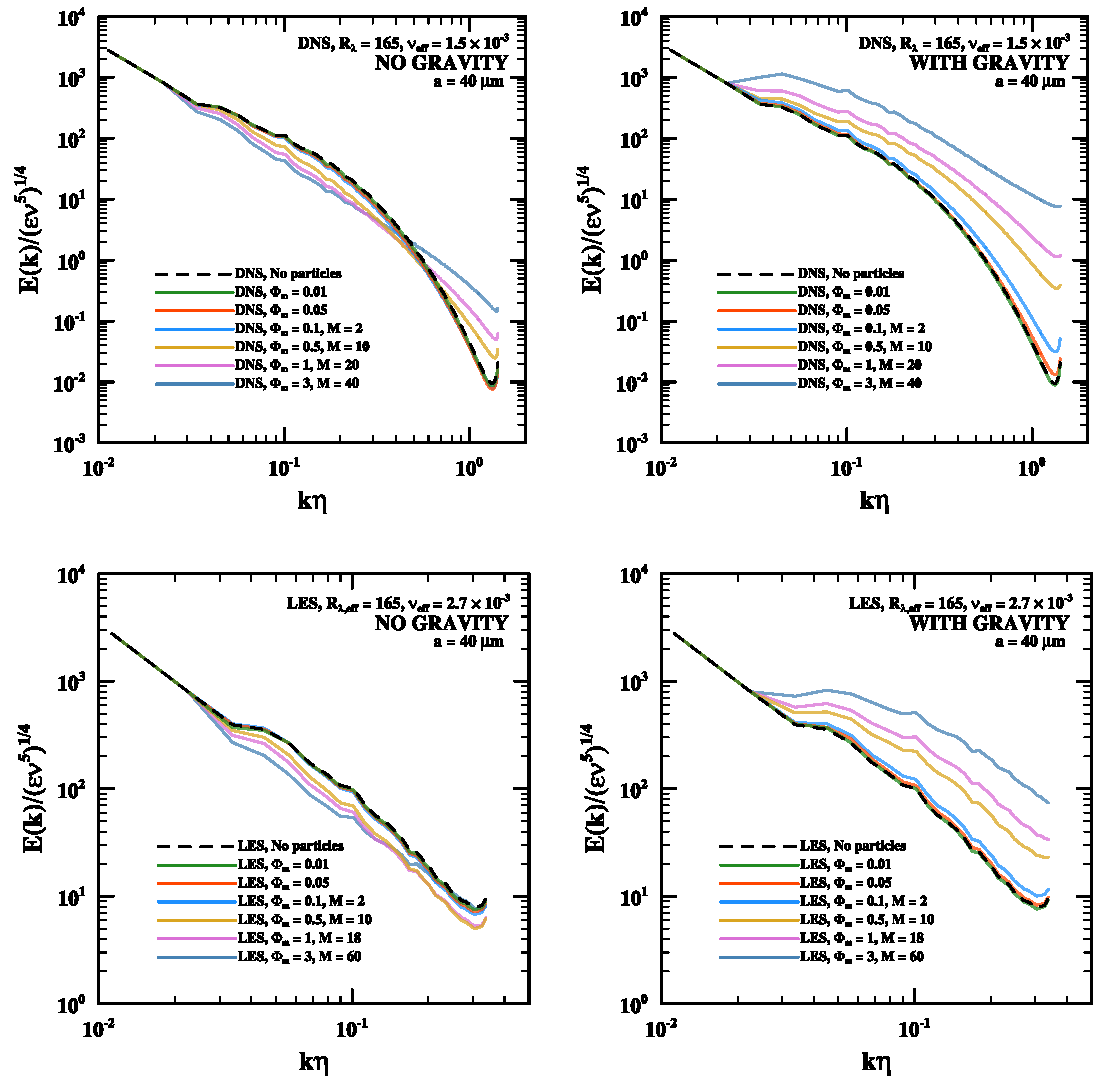
\includegraphics[width=13.5cm]{figures/2-03_modspec.pdf}
\caption{
The normalised energy spectra of turbulent flows with droplets of radii $40$~$\upmu\text{m}$, with and without gravity, as obtained using both DNS and LES with two-way momentum coupling and different particle mass loadings.
Dashed lines represent spectra without turbulence modulation by particles (see Figure \ref{fig:spec}).
For comparison (with DNS results only), see \textcite[Figure 4 therein]{Rosa2020}.
}
\label{fig:modspec}
\end{figure}

% FIGURE 2-04 - DISSIPATION SPECTRA OF TURBULENT FLOWS MODULATED BY PARTICLES
    
\begin{figure}
\centering
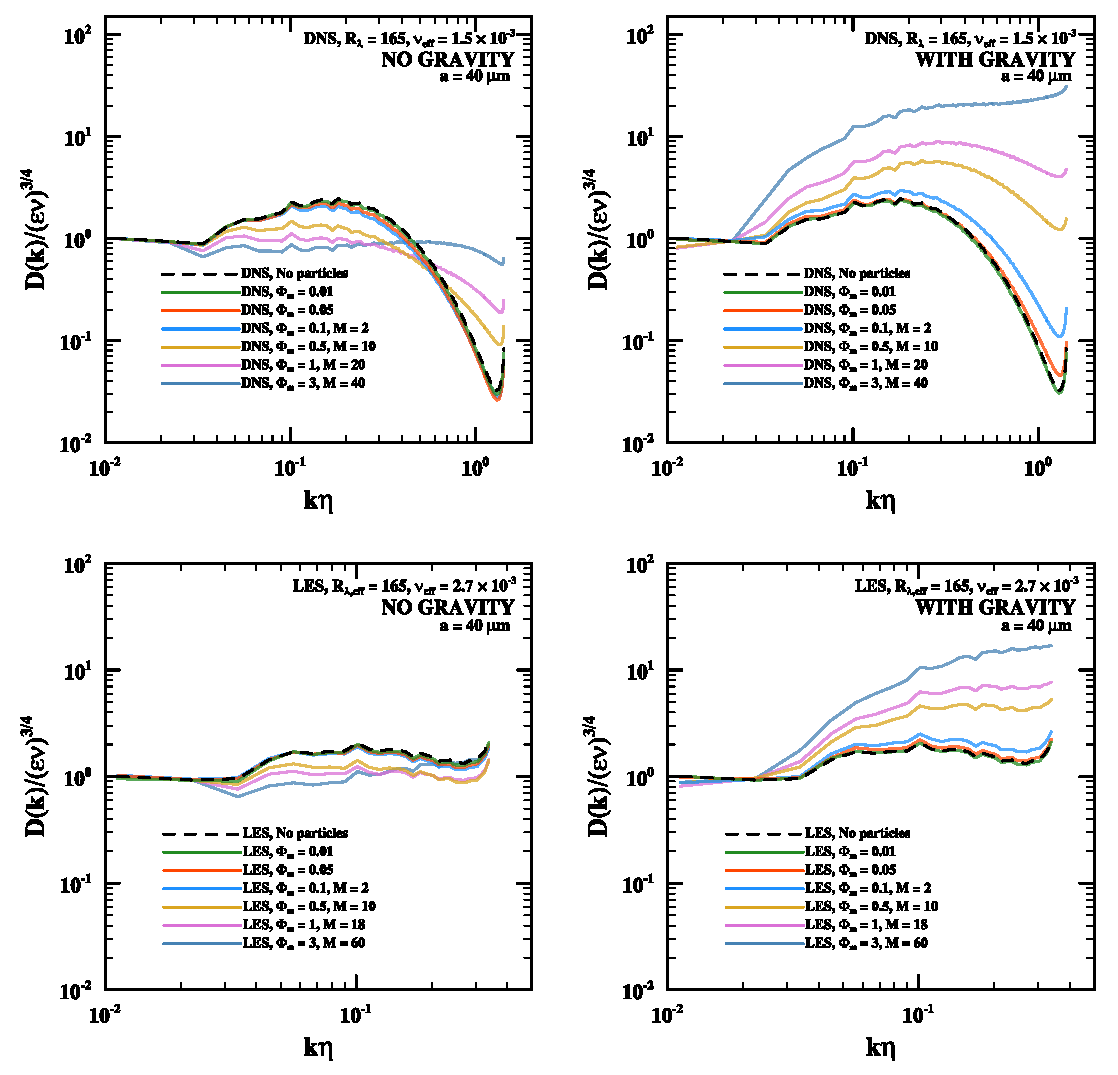
\includegraphics[width=13.5cm]{figures/2-04_moddiss.pdf}
\caption{
The normalised energy dissipation spectra of turbulent flows with droplets of radii $40$~$\upmu\text{m}$, with and without gravity, as obtained using both DNS and LES performed under two-way momentum coupling with different particle mass loadings.
Dashed lines represent dissipation spectra without turbulence modulation by particles (see Figure \ref{fig:diss}).
For comparison (DNS only), see Figure 5 in \textcite{Rosa2020}.
}
\label{fig:moddiss}
\end{figure}

% FIGURE 2-05 - PARAMETERS OF TURBULENT FLOWS MODULATED BY PARTICLES

\begin{figure}
\centering
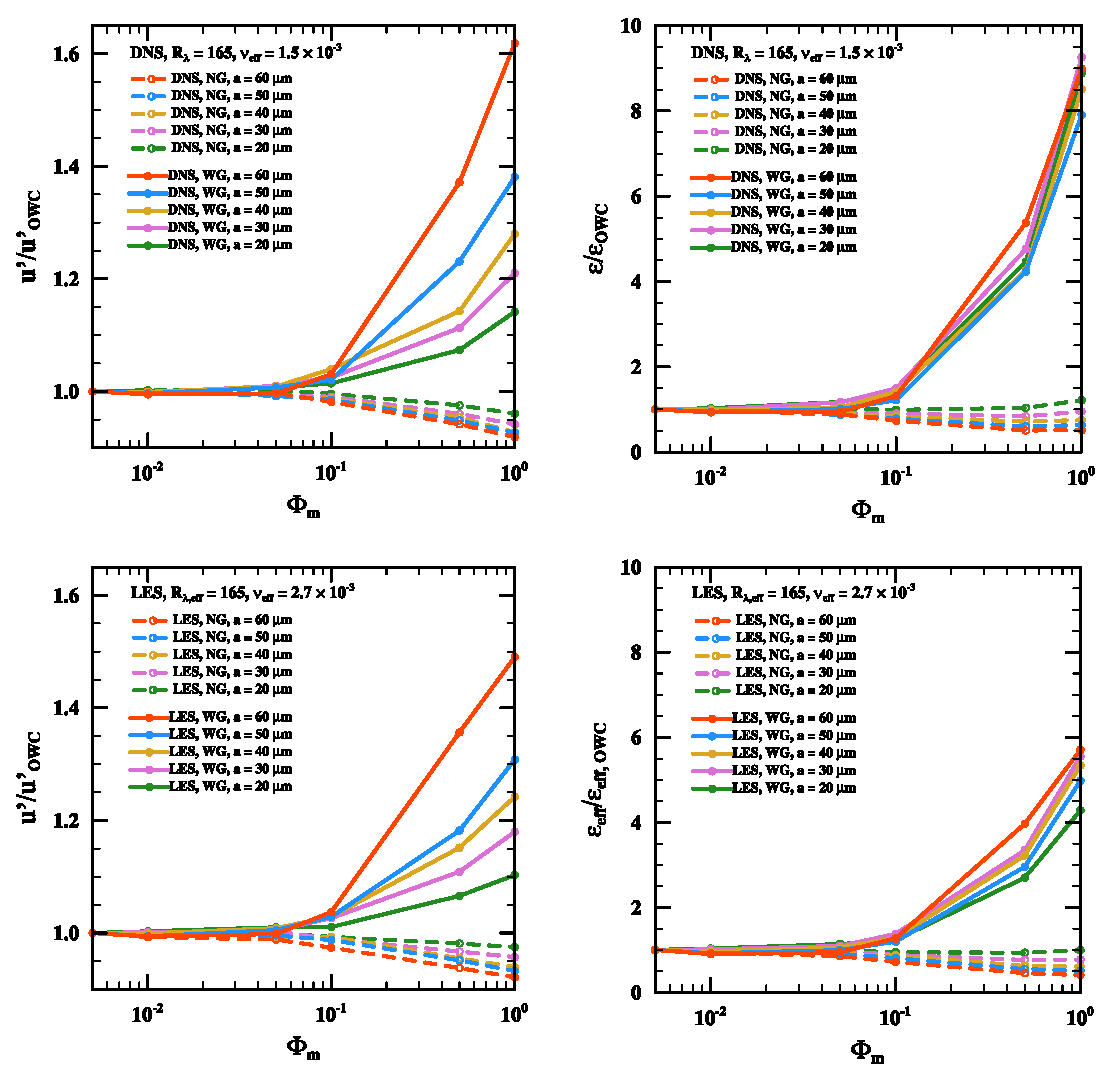
\includegraphics[width=13.5cm]{figures/2-05_modstat.pdf}
\caption{
Time averaged statistics of turbulent flows as obtained by DNS and LES under two-way momentum coupling, normalised by the corresponding statistics from simulations without turbulence modulation (OWC).
Plotted statistics include: the effective energy dissipation rate, $\epsilon_{\text{eff}}$ (top figures for DNS and LES, respectively), and the RMS fluctuating velocity, $u'$ (bottom figures, likewise).
WG denotes simulations with gravity (continuous lines); NG -- without gravity (dashed lines).
For comparison (DNS only), see Figure 11 in \textcite{Rosa2020}.
}
\label{fig:modstat}
\end{figure}

% FIGURE 2-06 - RDF AND RRV FOR OWC SIMULATIONS

\begin{figure}
\centering
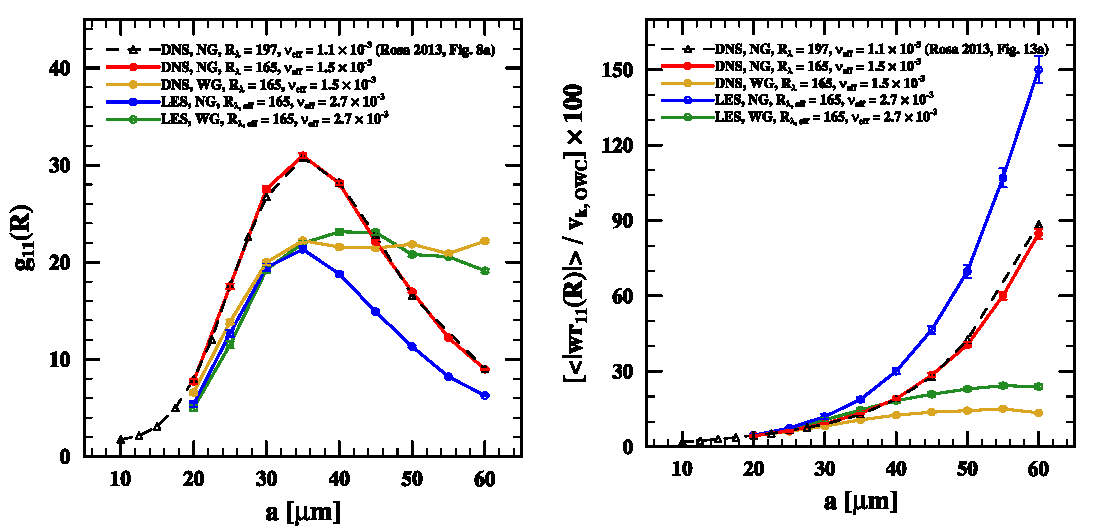
\includegraphics[width=13.5cm]{figures/2-06_owcrdfrrv.pdf}
\caption{
The values of the radial distribution function (RDF, left) and the radial relative velocity (RRV, right) at contact distance for simulations under one-way momentum coupling.
Results include data from both DNS and LES simulations, with (WG) and without (NG) gravity.
}
\label{fig:owcrdfrrv}
\end{figure}

% FIGURE 2-07 - COLLISON KERNELS FOR OWC SIMULATIONS

\begin{figure}[h]
\centering
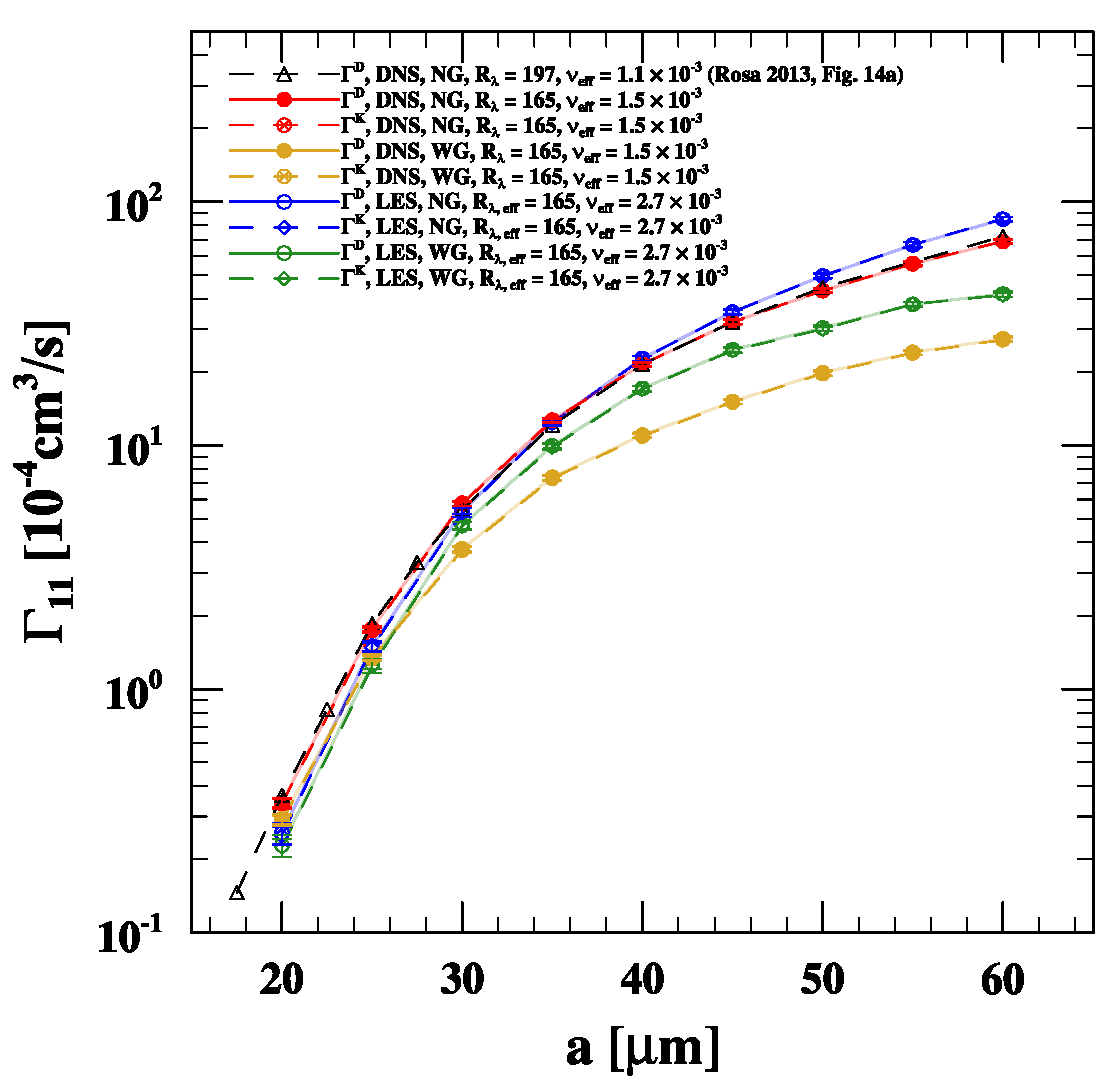
\includegraphics[width=10cm]{figures/2-07_owcgamma.pdf}
\caption{
The values of both dynamic and kinematic collision kernels for simulations under one-way momentum coupling.
Results include data from both DNS and LES simulations, with (WG) and without (NG) gravity.
Continuous lines represent values for dynamic kernel ($\Gamma_{11}^D$) and dashed ones (almost overlaid on continuous ones due to their close agreement) -- for kinematic kernel ($\Gamma_{11}^K$). 
}
\label{fig:owcgamma}
\end{figure}

% FIGURE 2-08 - RDF FOR TWC SIMULATIONS

\begin{figure}
\centering
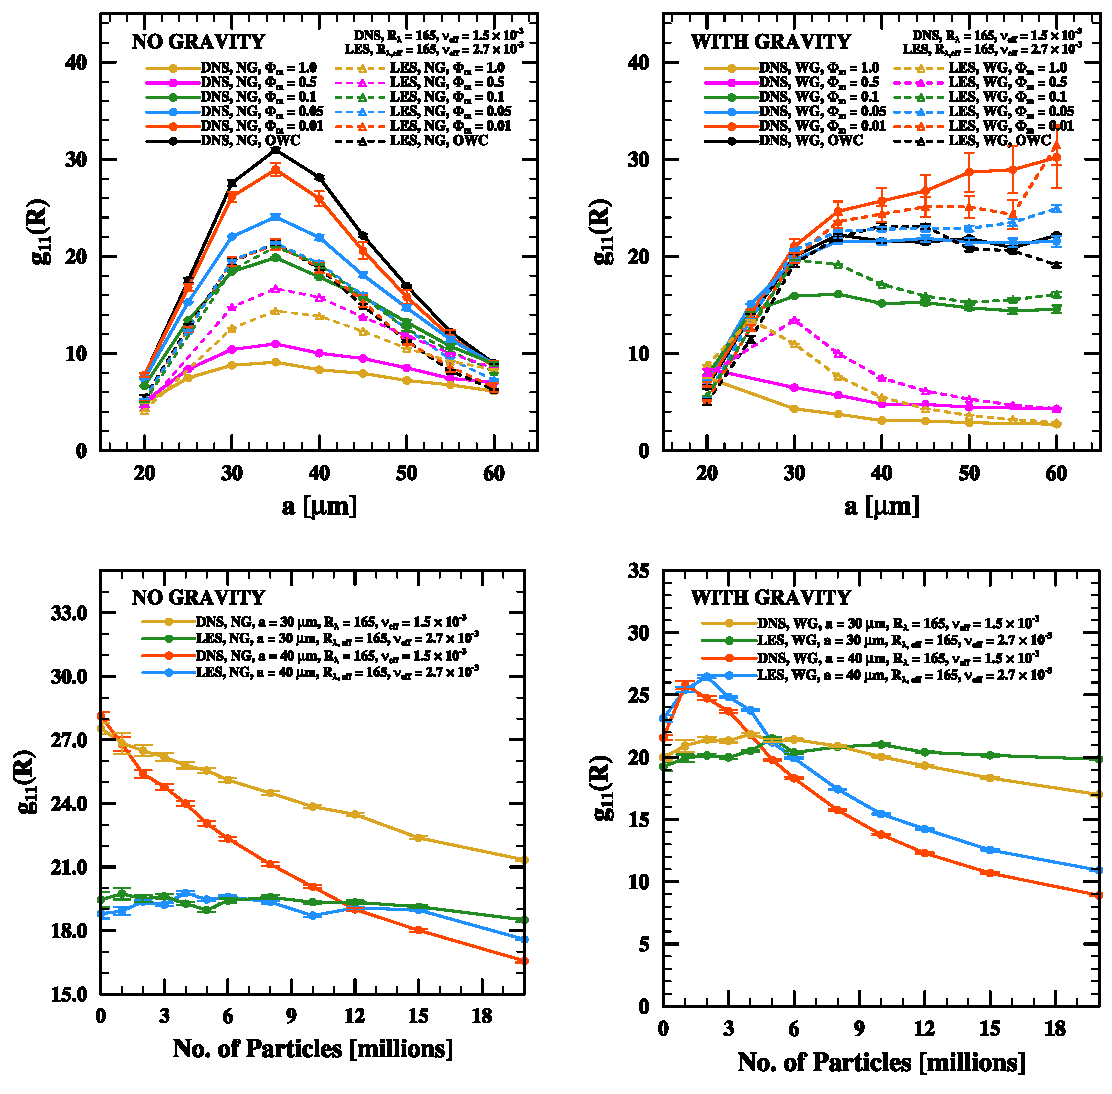
\includegraphics[width=13.5cm]{figuress/2-08_twcrdf.pdf}
\caption{
The values of radial distribution function (RDF) at contact distance for simulations under two-way momentum coupling using both DNS and LES.
Top plots show relation of RDF on particle radius for several fixed values of mass loading, $\Phi_m$ (also compared with results for OWC).
Bottom ones show the dependence of RDF on the number of particles (in millions) for particles with radii $30$~$\upmu\text{m}$ and $40$~$\upmu\text{m}$.
Plots on the left show results without effects of gravity (NG), and those on the right consider settling particles (WG).
}
\label{fig:twcrdf}
\end{figure}

% FIGURE 2-09 - RDF FOR TWC SIMULATIONS WITH LARGER MASS LOADINGS

\begin{figure}
\centering
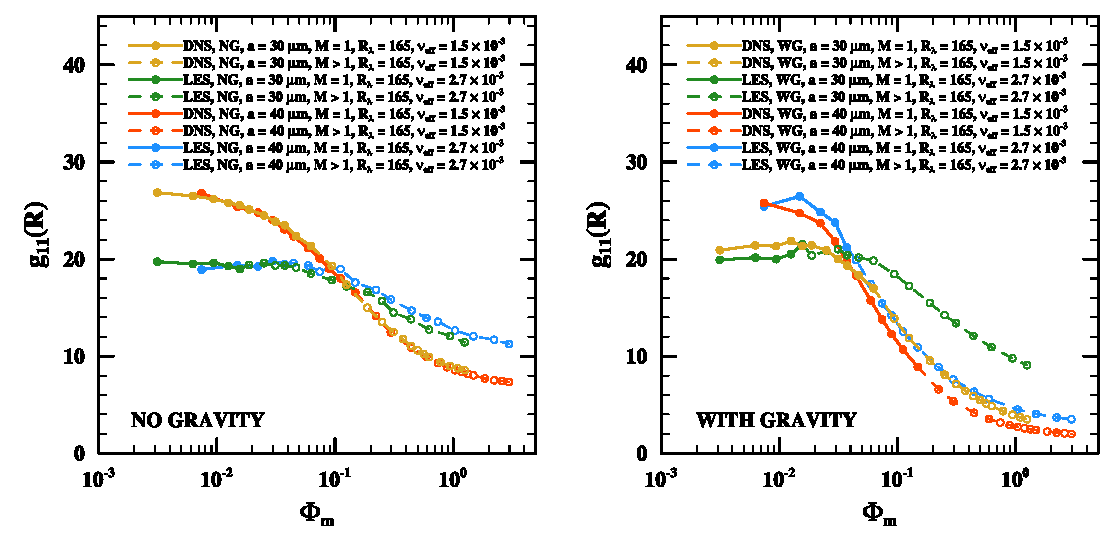
\includegraphics[width=13.5cm]{figures/2-09_twcrdfext.pdf}
\caption{
The values of RDF for wider range of mass loadings.
It may be considered as an extension of bottom plots from Figure \ref{fig:twcrdf} where scope was limited to $20$ million particles (${\Phi_m \approx 0.1}$).
Here, results include wider range of mass loadings where TWC should be most prominent (i.e. around $0.1$ to $1$) and where it may even not be sufficient (i.e. four-way coupling regime for $\Phi_m > 1$).
Continuous lines represent simulations without super-particle parameterisation ($M=1$), while dashed ones show where super-particle parameterisation was necessary to obtain larger mass loadings.
For precise information on values of $M$ for each simulation, see Appendix \ref{app:spp}. 
}
\label{fig:twcrdfext}
\end{figure}

% FIGURE 2-10 - RRV FOR TWC SIMULATIONS

\begin{figure}
\centering
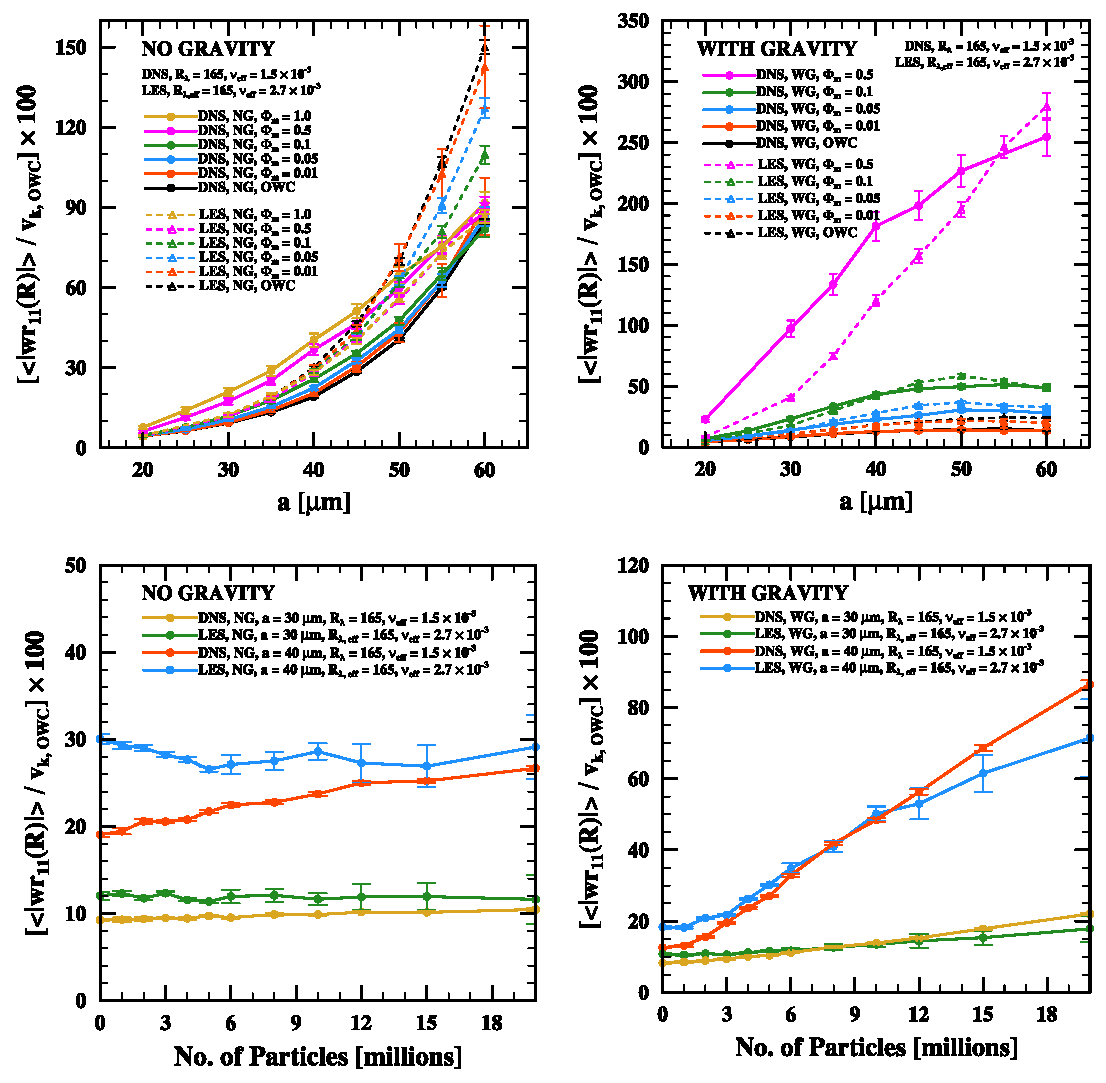
\includegraphics[width=13.5cm]{figures/2-10_twcrrv.pdf}
\caption{
The values of radial relative velocity (RRV) at contact distance for simulations under two-way momentum coupling using both DNS and LES.
Consistent with Figure \ref{fig:twcrdf}.
}
\label{fig:twcrrv}
\end{figure}

% FIGURE 2-11 - RRV FOR TWC SIMULATIONS WITH LARGER MASS LOADINGS

\begin{figure}
\centering
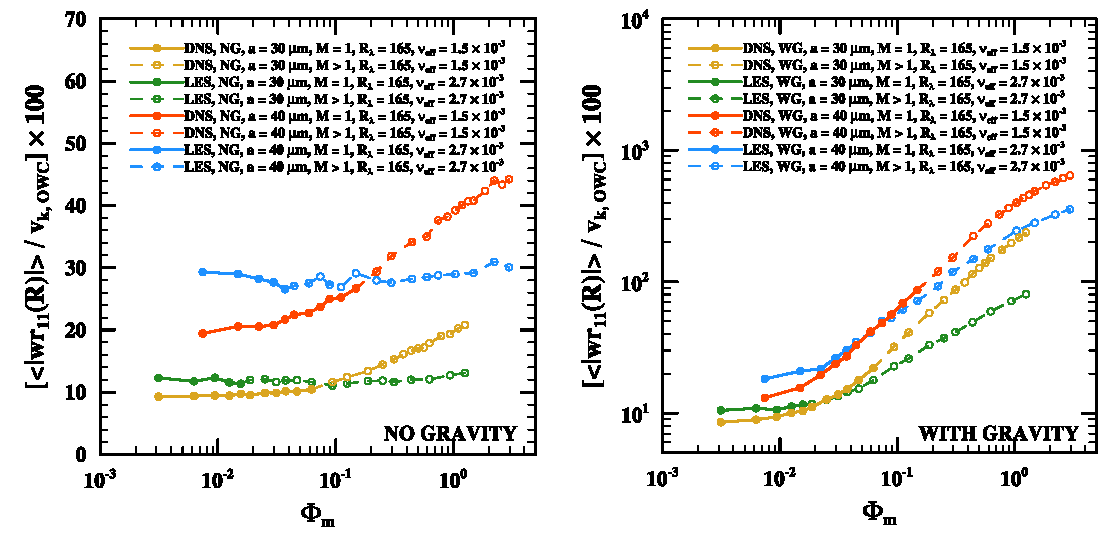
\includegraphics[width=13.5cm]{figures/2-11_twcrrvext.pdf}
\caption{
The values of RRV for wider range of mass loadings.
Consistent with Figure \ref{fig:twcrdfext}.
}
\label{fig:twcrrvext}
\end{figure}

% FIGURE 2-12 - DYNAMIC COLLISION KERNELS FOR TWC SIMULATIONS

\begin{figure}
\centering
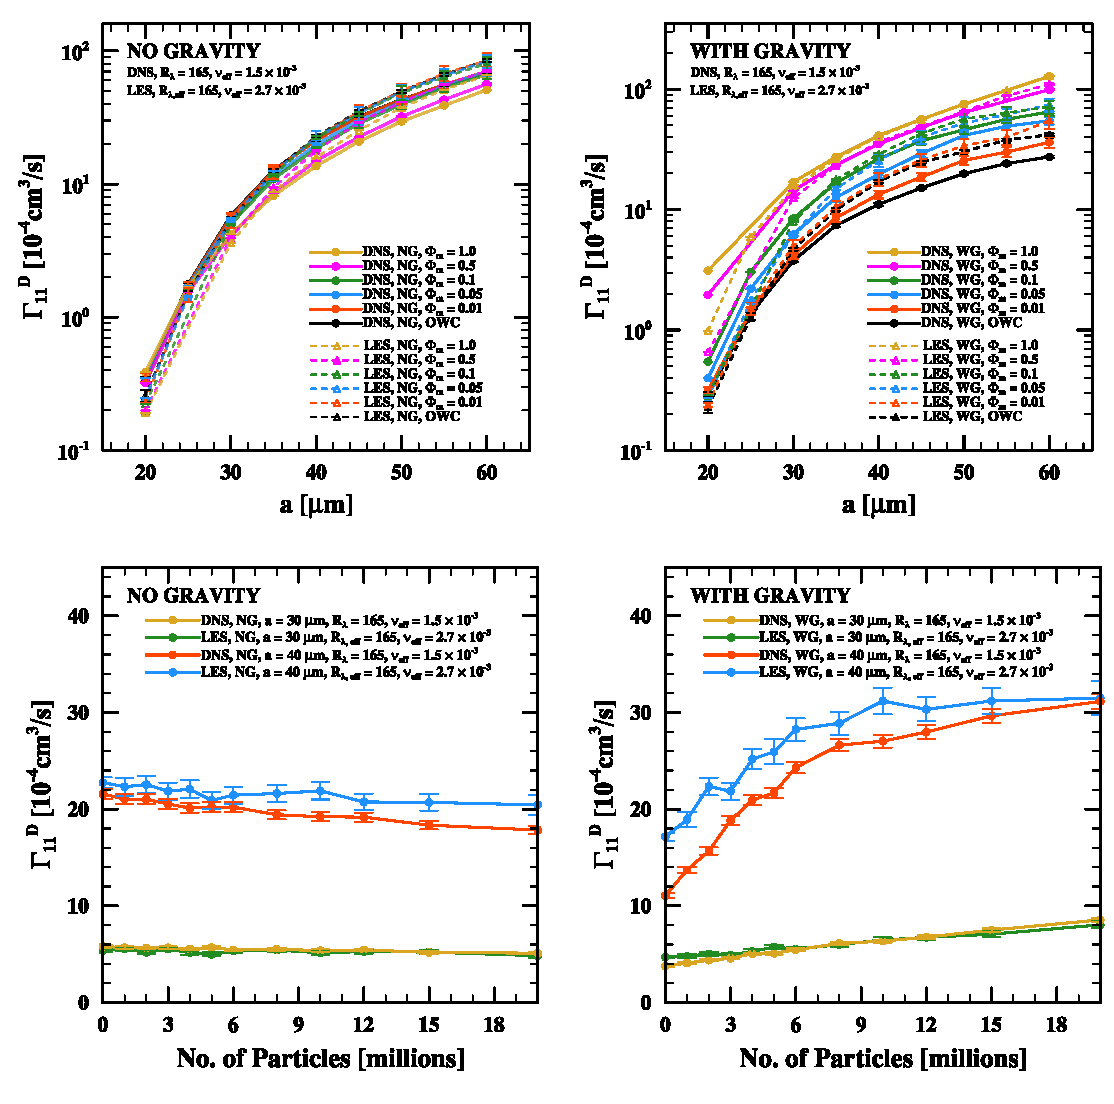
\includegraphics[width=13.5cm]{figures/2-12_twcgamma.pdf}
\caption{
The values of dynamic collision kernel ($\Gamma_{11}^D$) for simulations under two-way momentum coupling using both DNS and LES.
Consistent with Figure \ref{fig:twcrdf}.
}
\label{fig:twcgamma}
\end{figure}

% FIGURE 2-13 - DYNAMIC COLLISION KERNELS FOR SIMULATIONS WITH LARGER MASS LOADINGS

\begin{figure}[h]
\centering
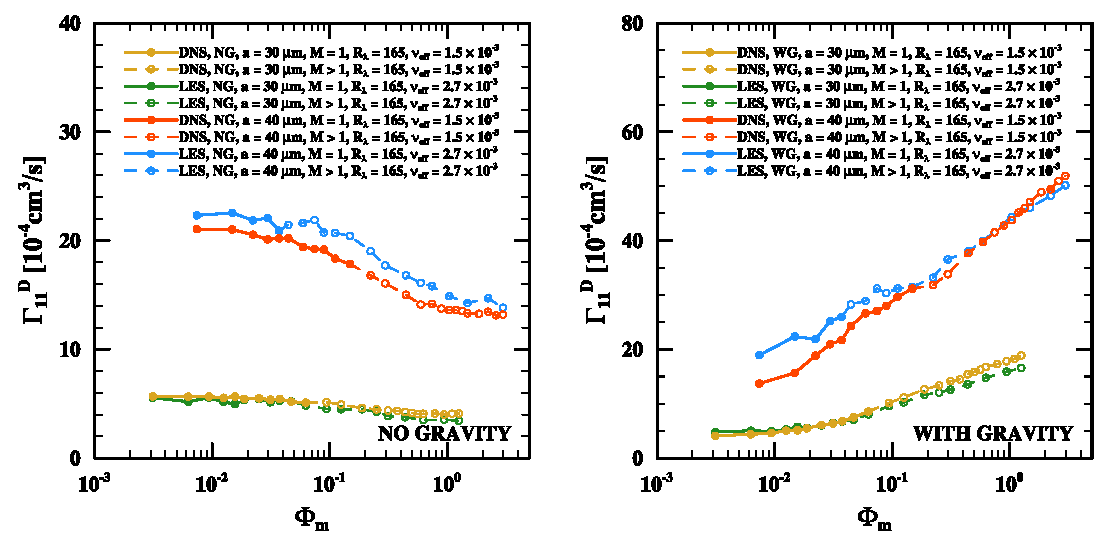
\includegraphics[width=13.5cm]{figures/2-13_twcgammaext.pdf}
\caption{
The values of dynamic collision kernel for wider range of mass loadings.
Consistent with Figure \ref{fig:twcrdfext}.
}
\label{fig:twcgammaext}
\end{figure}
    

